\chapter{Pre-training losses}
\label{sec:app2}

This chapter shows two exemplary loss curves during the pre-training. They have not been shown in the main part. However, one can observe the dependency of the adversary on the classifier. Secondly it can be seen that the adversary does not affect the classifier. 

\begin{figure}[h]
	\centering
	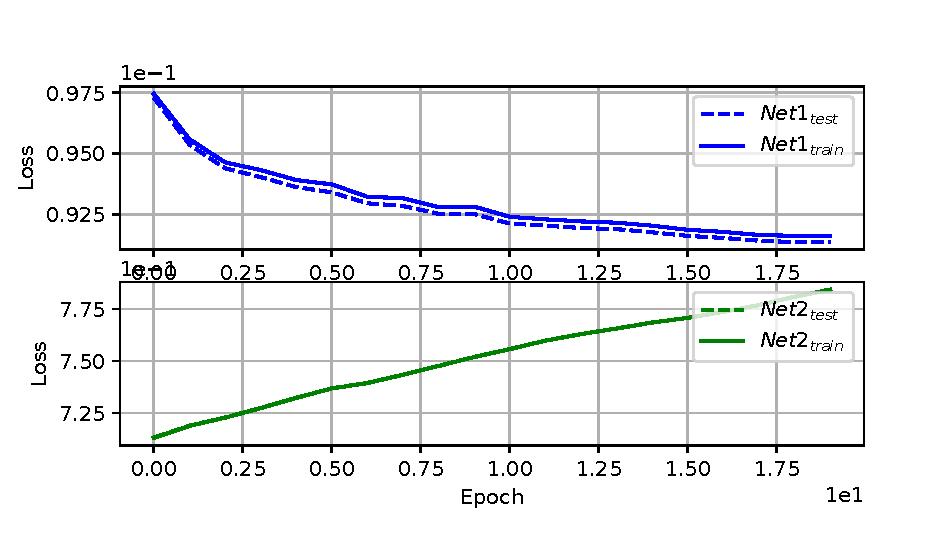
\includegraphics[width=\textwidth]{D_pretrain}
	\caption[Classifier pretraining]{Pre-training of the classifier. It is visible that even a normal training worsens the adversary's performance. It also indicates that the adversary really depends on the classifier.}
	\label{fig:D_pre}
\end{figure}

\begin{figure}[h]
	\centering
	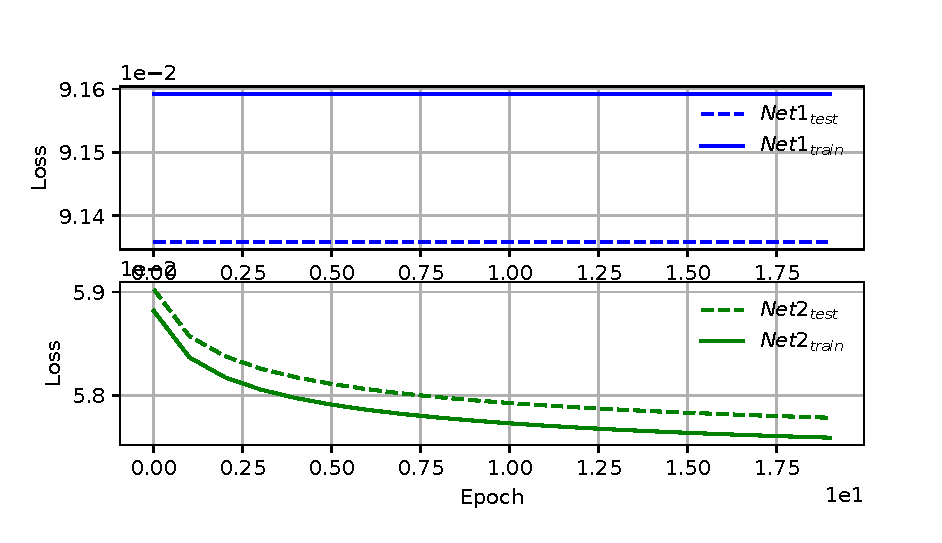
\includegraphics[width=\textwidth]{R_pretrain}
	\caption[Adversary pretraining]{Pre-training of the adversary. It is visible, that the adversary does not affect the classifier directly.}
	\label{fig:R_pre}
\end{figure}